\chapter{Funktionsweise \label{chap_funktionsweise}}
\ac{ITS} besteht aus verschiedenen Komponenten. Diese Komponenten können mobil oder stationär sein. Die Grafik \ref{fig:funktionsweise_komponentenueberblick} gibt einen Überblick über die in \ac{ITS} verwendeten Komponenten. Jede dieser Komponenten enthält eine \ac{ITS} Station. Dieser Abschnitt bezieht sich hauptsächlich auf die ETSIStandards \cite{etsi2010302} und \cite{etsi302636-3}. Standard \cite{etsi2010302} definiert Funktionalitäten, Standard  \cite{etsi302636-3} definiert die Realisierung dieser Funktionalitäten. Im Folgenden werden die Komponenten beschrieben und anhand von beiden Standards erklärt.


\begin{figure}
	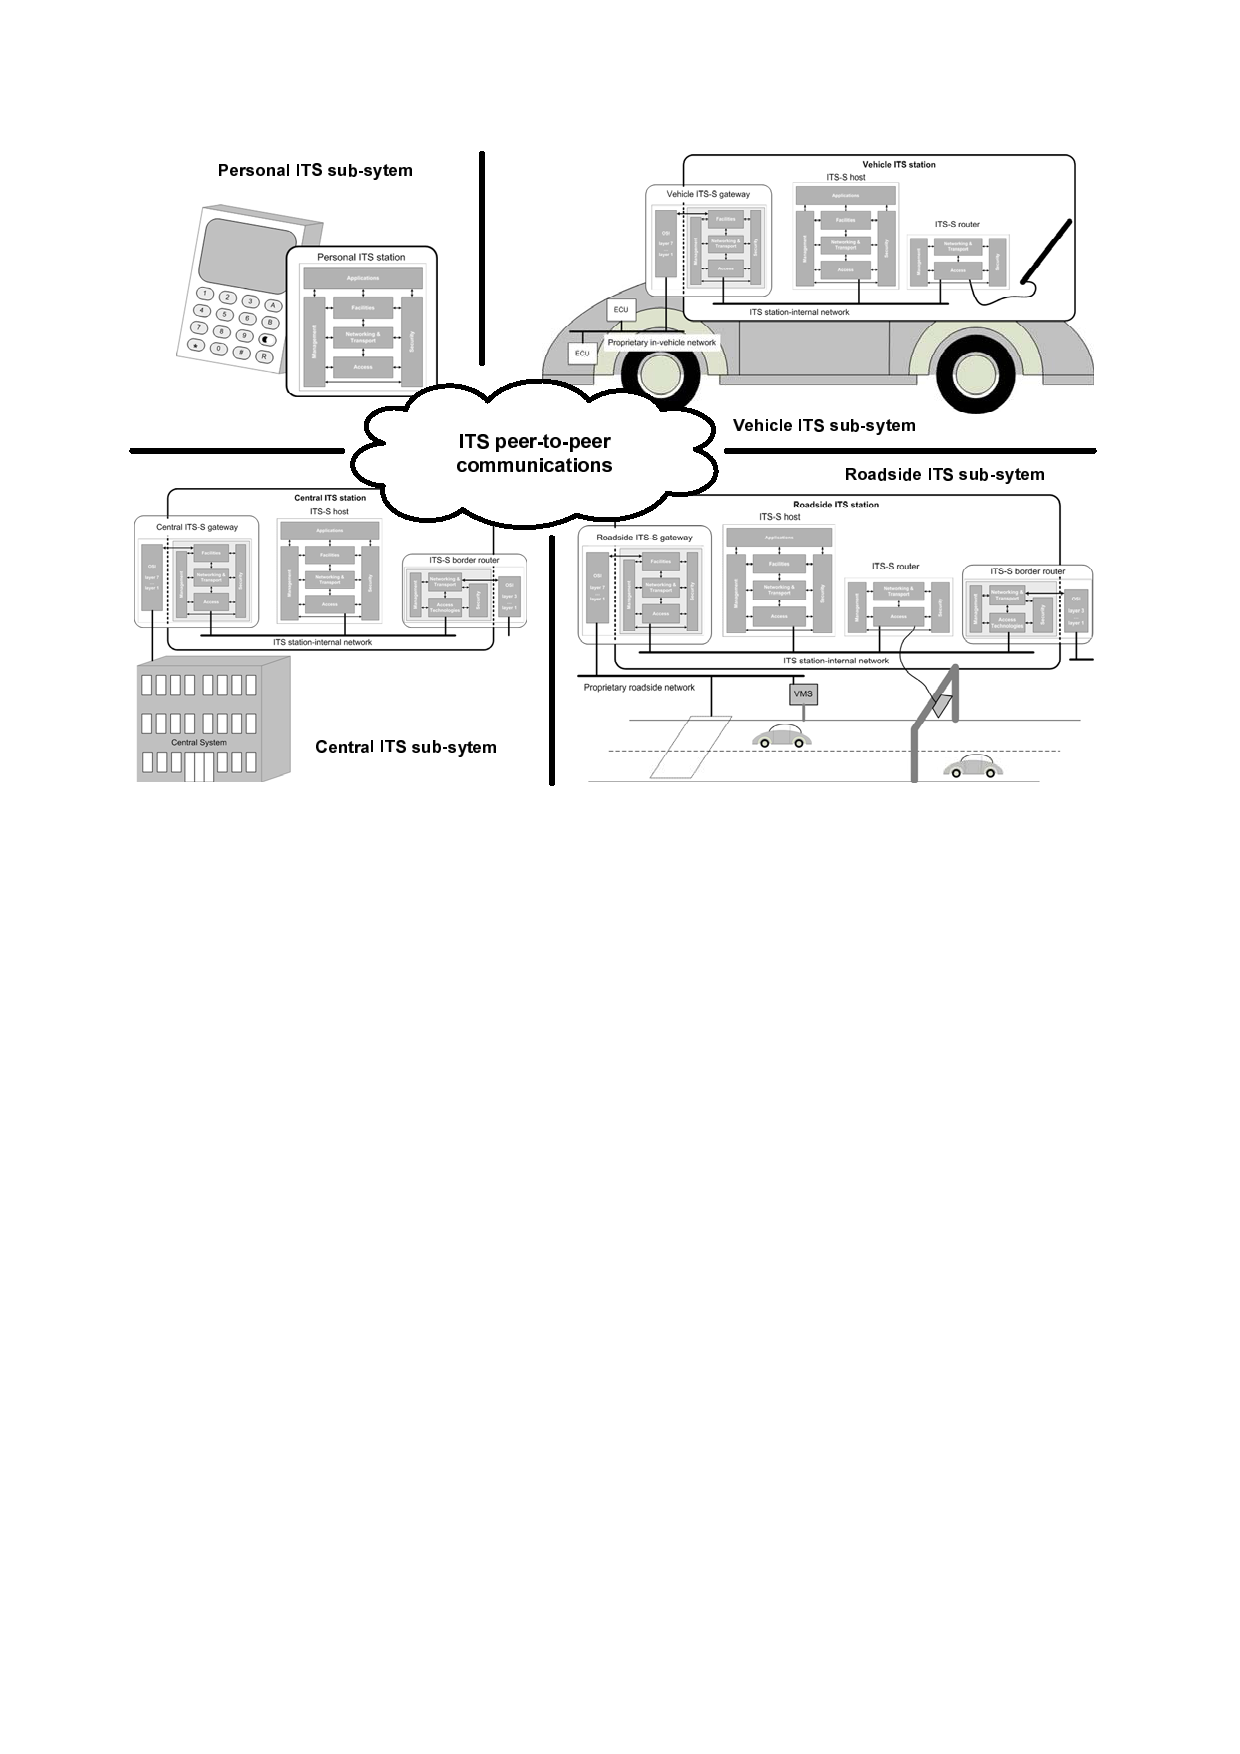
\includegraphics[width=0.99\textwidth]{content/images/01_funktionsweise/ueberblick-ITS-subsystems.pdf}
	\caption{Überblick über die Komponenten \cite{etsi2010302}}
	\label{fig:funktionsweise_komponentenueberblick}
\end{figure}


\section{Funktionale Komponenten von ITS \label{funktionsweise_funktionaleKomponenten}}
Die funktionalen Komponenten sind sind in sich geschlossene Einheiten, die in den \ac{ITS} Untersystemenen vorhanden sind. Sie werden in diesem Abschnitt beschrieben. Zusätzlich werden die mindestens definierten Funktionalitäten genannt.

Auf die einzelnen Layer der Komponenten wird im Kapitel \ref{chap_archtitektur} eingegangen.   

Die einzelnen funktionalen Komponenten müssen nicht physikalisch getrennt werden. Es reicht eine logische Trennung.  

\subsection{ITS-S Host \label{funktionsweise_ITSHost}}
Der ITS-S Host beinhaltet mindestens die ITS-S Anwendungen und die Funktionalität der ITS  Station Reference Architektur, die für die  ITS-S Anwendungen gebraucht wird. Konkret sind das der \ac{ITS} Network Layer und die Anwendungsebene. 

Die Funktionalitäten des ITS-S Host werden im Standard \cite{etsi302636-3} der \ac{AU} zugesprochen. Sämtliche andere Funktionalitäten sind auf die \ac{CCU} ausgelagert. Diese Aufteilung hängt aber von der zu implementierenden Komponente ab, ein Skalieren muss möglich sein.

\subsection{Roadside ITS-S Gateway \label{funktionsweise_RoadsideITSGateway}}
Die Funktionsweise des Roadside ITS-S Gateway ergibt sich aus der Grafik \ref{fig:funktionsweise_itsGateway}. Die Aufgabe ist die gleiche, wie bei den meisten Gateways. Es verbindet unterschiedliche Protokollstacks miteinander. In diesem Fall werden das \ac{ITS} interne Netzwerk und ein proprietäres Netzwerk miteinander verbunden. Das proprietäre Netzwerk kann beispielsweise ein IP basierendes Netzwerk sein.

\begin{figure}[h]
	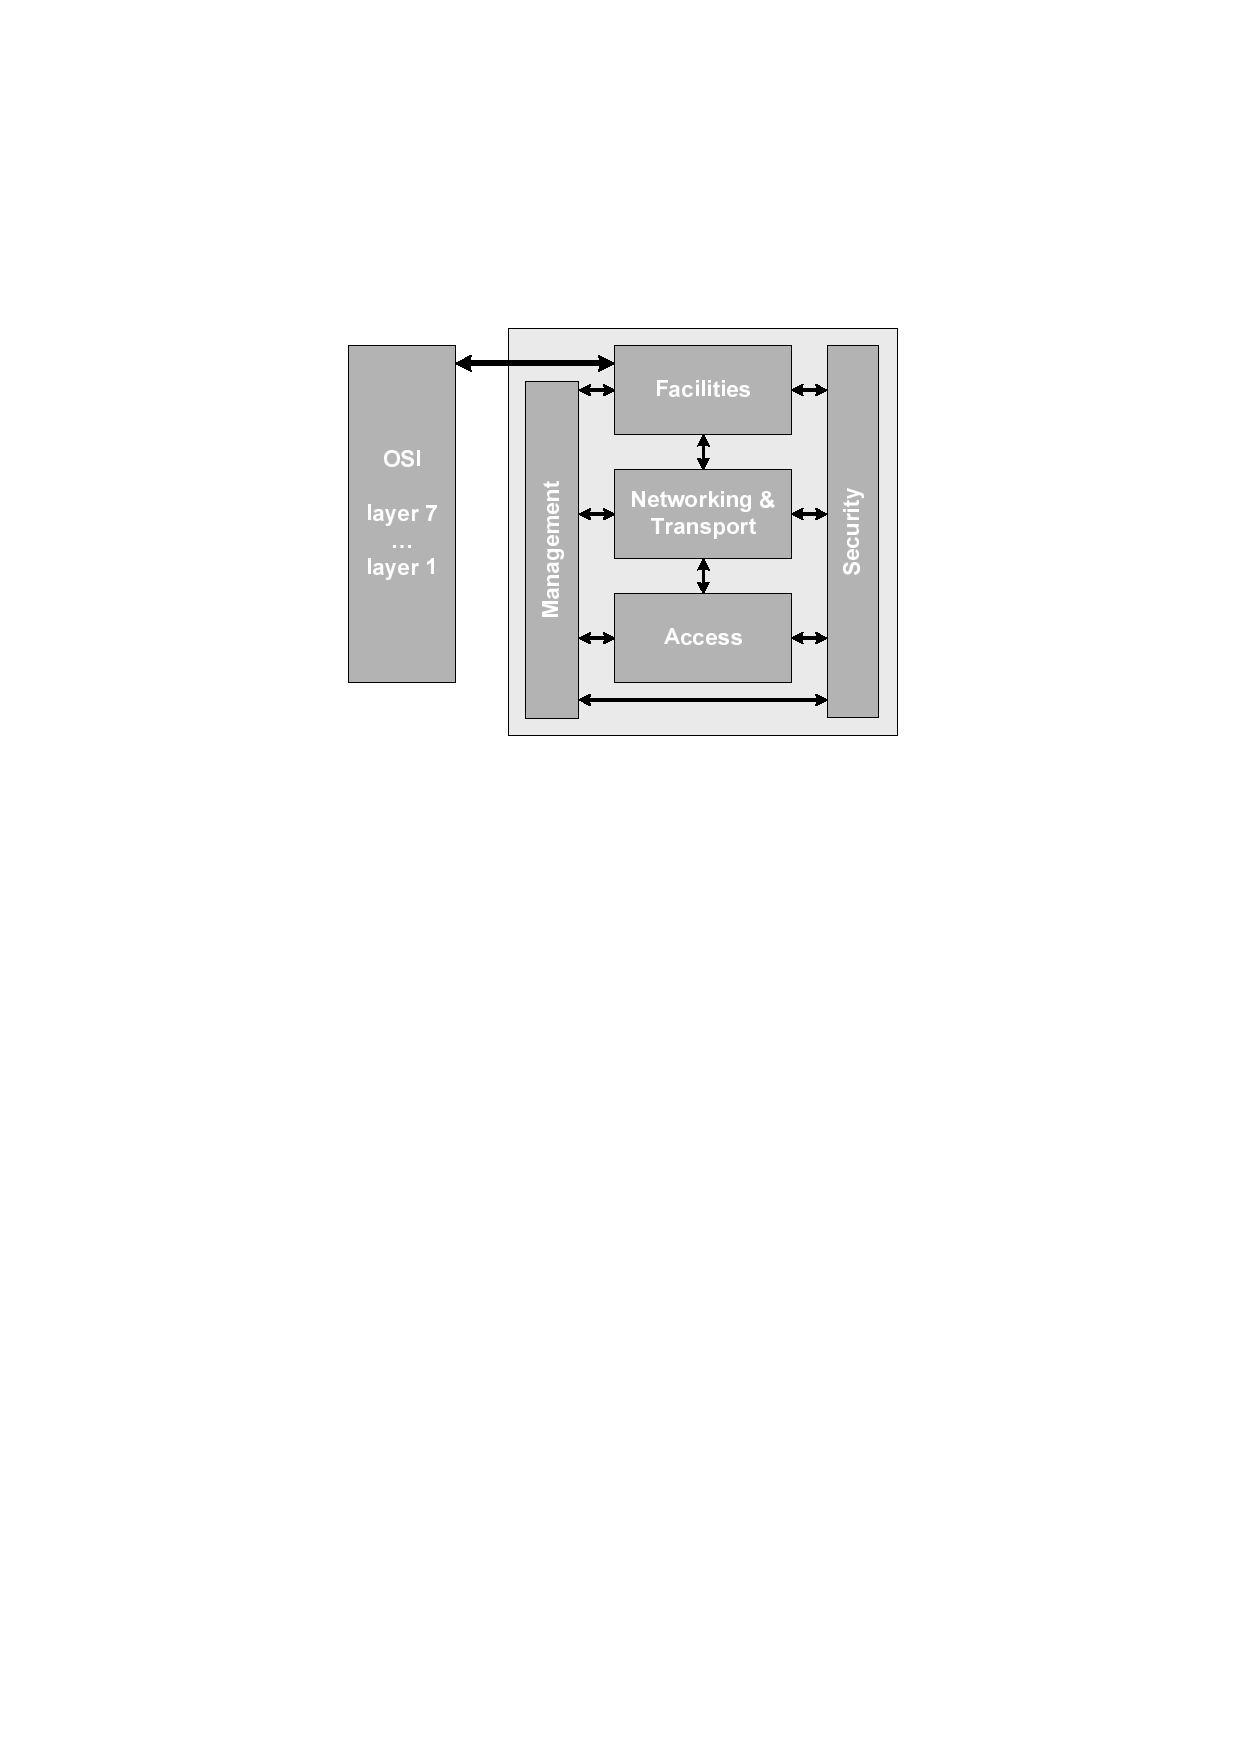
\includegraphics[width=0.75\textwidth]{content/images/01_funktionsweise/layer_gateway.pdf}
	\caption{Überblick über die Layer eines ITS Gateways \cite{etsi2010302}}
	\label{fig:funktionsweise_itsGateway}
\end{figure}


\subsection{ITS-S Router \label{funktionsweise_router}}
Ein \ac{ITS} Router bietet alle Funktionen der \ac{ISO} Referenzarchitektur, ausgenommen die beiden oberen Layer Application und Facilities. Er verbindet zwei unterschiedliche \ac{ITS} Protokoll Stacks auf Layer 3. Einer dieser Protokoll Stacks ist normalerweise mit dem internen \ac{ITS} Netzwerk verbunden. Router werden genutzt um eine Verbindung zu anderen \ac{ITS} Komponenten aufzubauen. Die Darstellung der Layer eines Routers befindet sich in Grafik  \ref{fig:funktionsweise_layerHost}.

\begin{figure}
	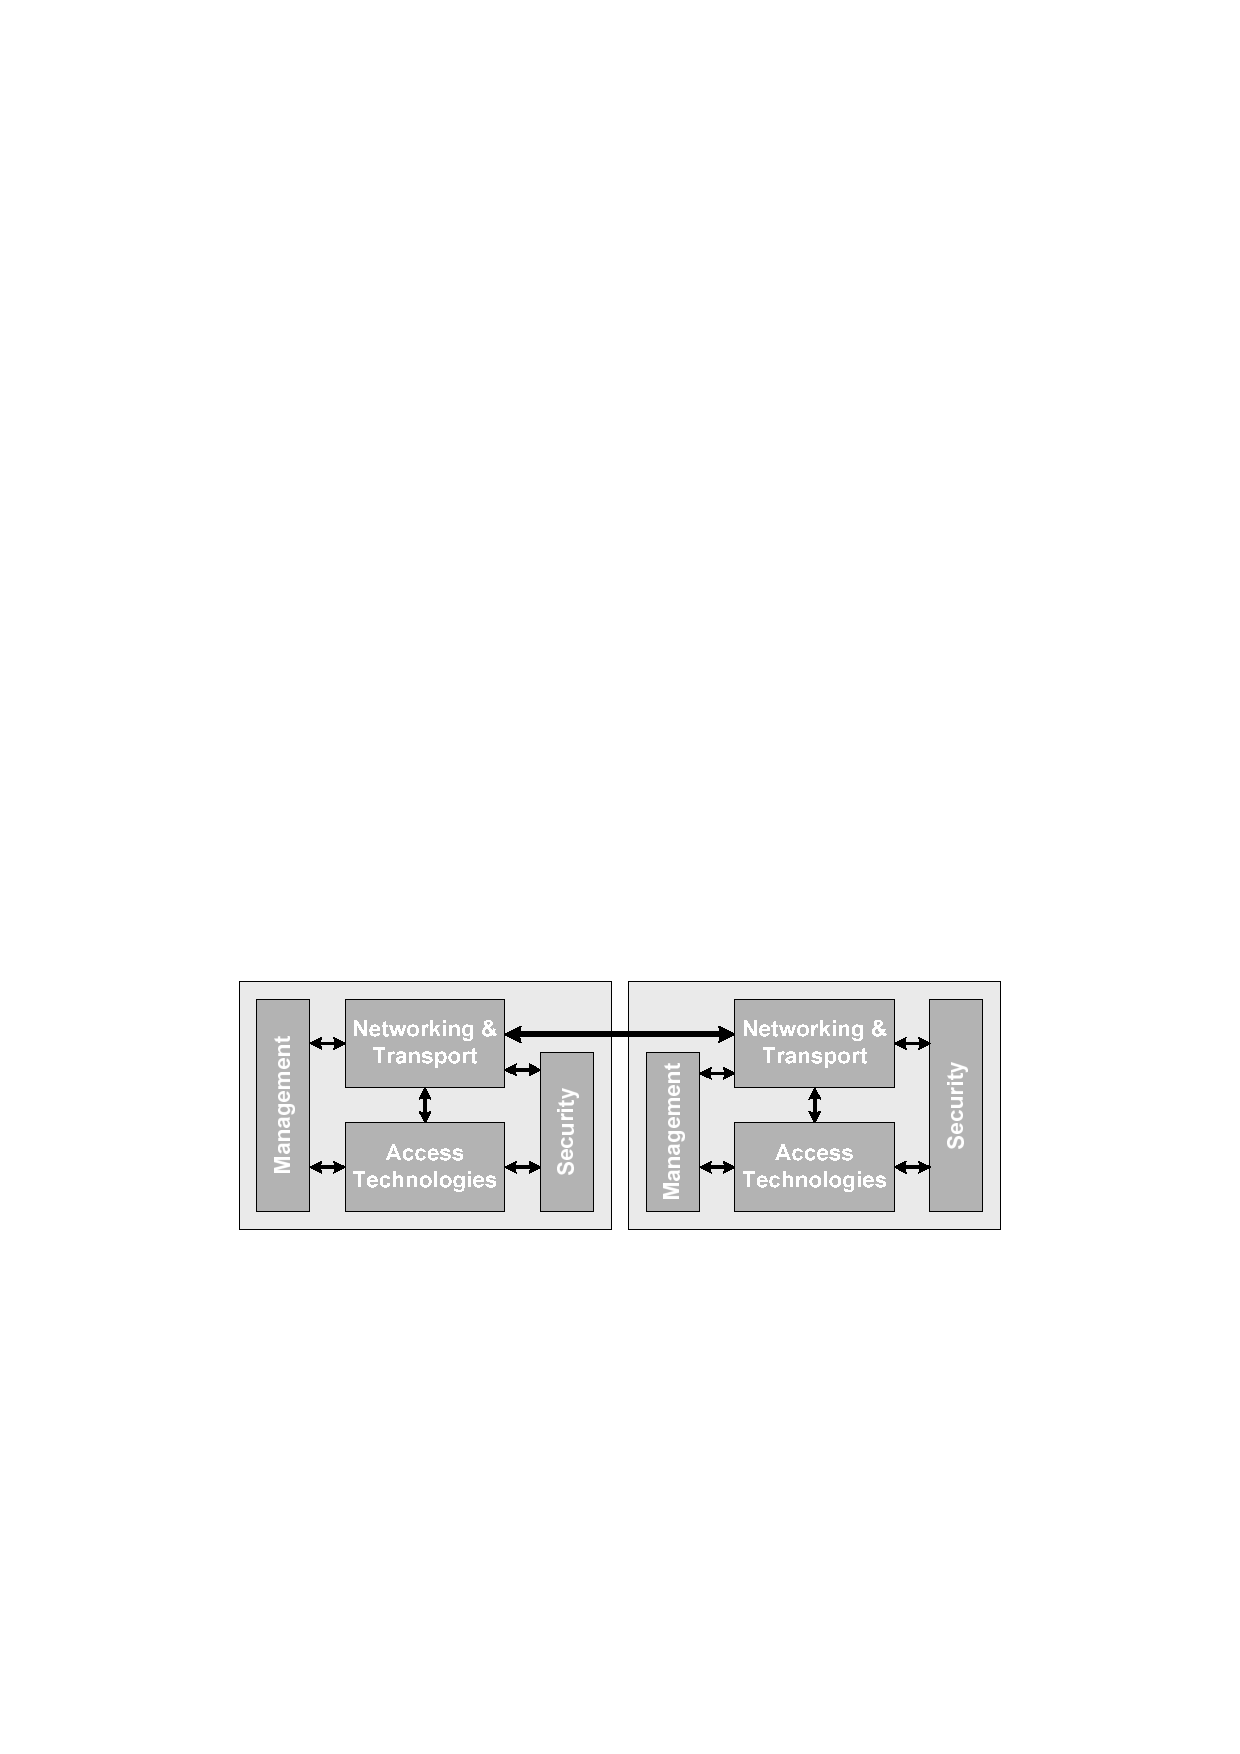
\includegraphics[width=0.99\textwidth]{content/images/01_funktionsweise/layer_router.pdf}
	\caption{Überblick über die Layer eines ITS Hosts \cite{etsi2010302}}
	\label{fig:funktionsweise_layerHost}
\end{figure}



\subsection{ITS-S Border Router \label{funktionsweise_ITSBorderRouter}}
Ein Border Router hat die gleichen Funktionalitäten wie ein Router \ref{funktionsweise_router}. Der Unterschied ist, dass ein Border Router zwischen einem \ac{ITS} Netz und einem Netz ohne die Cross Layer vermitteln kann. Ein Beispiel für ein solches Netz ist das Internet.

  
\begin{figure}
	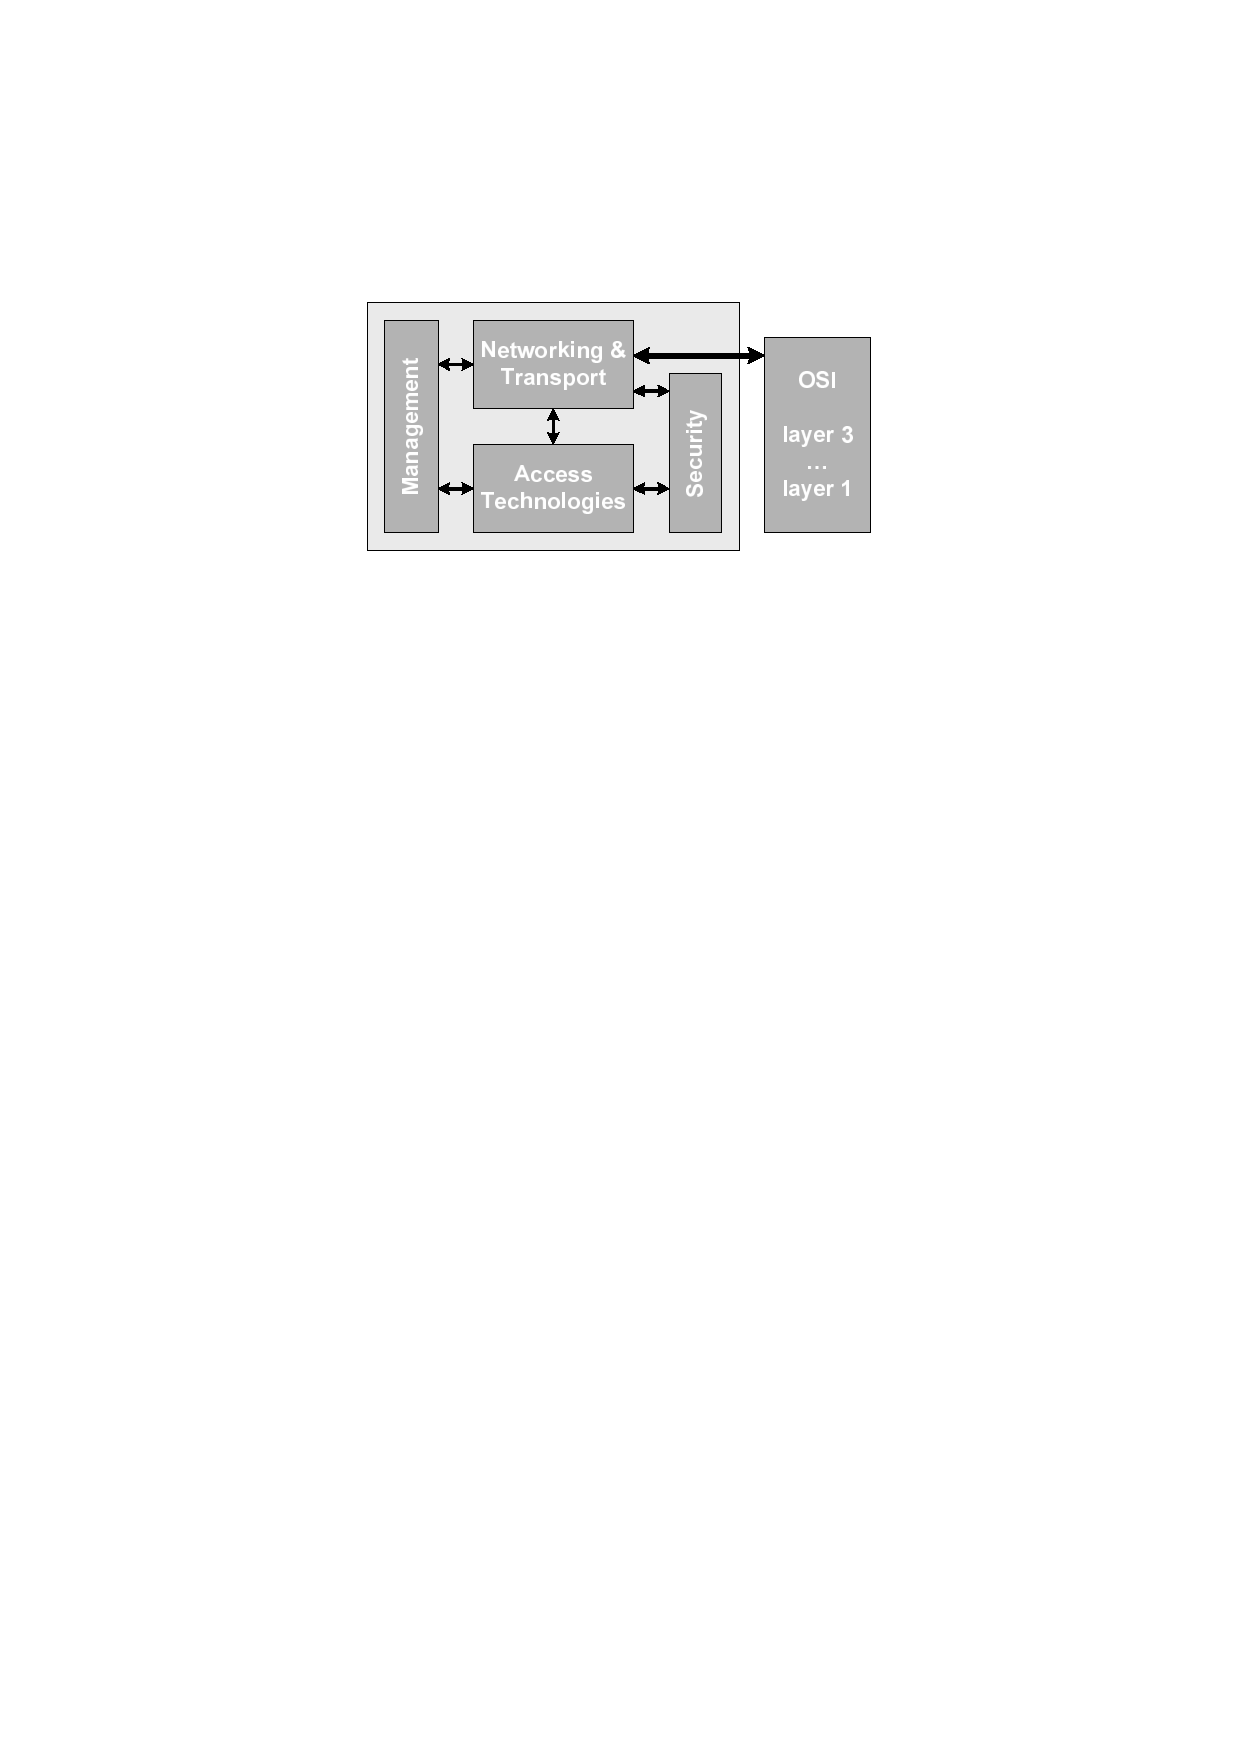
\includegraphics[width=0.99\textwidth]{content/images/01_funktionsweise/layer_borderRouter.pdf}
	\caption{Überblick über die Layer eines ITS Border Routers \cite{etsi2010302}}
	\label{fig:funktionsweise_borderRouter}
\end{figure}



\section{Personal subsystem and station}
\ac{PSS} stellen die Funktionalitäten von \ac{ITS} in Geräten zur Verfügung, die in der Hand gehalten werden können. Der Standard nennt hierzu \ac{PDA} oder Mobiltelefone als Beispiel. Sie können als eigenständige Komponente dienen, oder als Teil einer anderen Komponente arbeiten.
\todo{Für das PSS die funktionalen Komponenten suchen}

\section{ITS Central Station}
Die \ac{ICS}, oder Central \ac{ITS} subsystem and station ist eine zentrale Komponente im \ac{ITS} System. Sie bietet die Funktionalität an, um die Komponenten des zentralen Systems an das \ac{ITS} 

Die mindesten funktionalen Komponenten der \ac{ICS} sind:
\begin{itemize}
	\item ITS-S Gateway \ref{funktionsweise_RoadsideITSGateway}
	\item ITS-S Host \ref{funktionsweise_ITSHost}
	\item ITS-S Border Router \ref{funktionsweise_ITSBorderRouter}
\end{itemize}


Core component of the architecture is the ITS station, which has two main roles: in its first role, the ITS station is a network node and acts as a communication source or sink. Likewise an ITS station can be a forwarder of data, e.g. in the ITS ad hoc network. In its second role, the ITS station is placed at the network edge and connect the different networks via an ITS station internal network (see Figure 1). \cite{etsi302636-3}

\todo{Noch was zur ICS finden}
	
	
\section{ITS Roadside Station}
Die Kommunikation ist nicht auf die Kommunikation von Fahrzeugen untereinander beschränkt. Eine Kommunikation zwischen Fahrzeugen und Verkehrsinfrastruktur ist ebenfalls möglich. Diese Kommunikation wird über \ac{IRS} oder \ac{RSU} abgewickelt. Da sie den Informationsfluss zwischen \ac{IVS} und \ac{ICS} ermöglicht, hat sie einen hohen Stellenwert im System. \ac{IRS} werden im Normalfall in bereits vorhandene Infrastruktur integriert. Hierfür bieten sich beispielsweise Ampeln oder sonstige Verkehrsleitsysteme an. 

Die \ac{IRS} beherrscht zwei grundlegend unterschiedliche Verbindungsprotokolle. Über das verbindungslose ITS-G5 kann die \ac{IRS} Verbindungen zu den \ac{IVS} aufbauen. Die Verbindung zu den \ac{ICS} erfolgt über TCP/IP. 

Normalerweise besteht eine \ac{IRS} aus den funktionalen Komponenten: 
\begin{itemize}
	\item  ITS-S Gateway \ref{funktionsweise_RoadsideITSGateway}
	\item ITS-S Host \ref{funktionsweise_ITSHost}
	\item ITS-S Router \ref{funktionsweise_router}
	\item ITS-S Border Router \ref{funktionsweise_ITSBorderRouter}
\end{itemize}

Neben der Funktion als reine Schnittstelle zwischen \ac{IRS} und \ac{IVS} kann die \ac{IRS} die empfangenen Daten aufbereiten, bzw. ein FunctionFramework zur Verfügung stellen, auf dem Applikationen ausgeführt werden können. Die Funktionen des FunctionFramework sind in der Beschreibung des Hosts \ref{funktionsweise_ITSHost} definiert.  

Beispiele für Applikationen der \ac{IRS} sind:
\begin{itemize}
	\item Store and Forward von Ereignisinformationen \ac{DENM}
	\item Weiterleitung von Ereignisinformationen an Versuchszentrale (Testzentrale)
	\item Aggregation von empfangenen Fahrzeugdaten zur Verbesserung der Wetter- und Verkehrslageerfassung
	\item Neue Anwendungen bzgl. der Interaktion zwischen Fahrzeug und LSA
	\item  Kreuzungsassistenz sowie Assistenz im Baustellenbereich.
	\item Verteilung von Daten der ergänzenden Dienste aus der Versuchszentrale an die Fahrzeuge
	\item Versendung von Daten zur Kreuzungstopologie
\end{itemize}

Diese Beispiele sind aus einem Projektergebnis von \ac{SIMTD} entnommen (\cite{simtd-D12.1}). 



\section{IVS}
Das \ac{IVS} ist eine mobile Komponente von \ac{ITS}. Es hat als Mindestanforderung lediglich Schnittstellen in das \ac{ITS} Netzwerk. Es besteht mindestens aus folgenden funktionalen Komponenten:
\begin{itemize}
	\item  ITS-S Gateway \ref{funktionsweise_RoadsideITSGateway}
	\item ITS-S Host \ref{funktionsweise_ITSHost}
	\item ITS-S Router \ref{funktionsweise_router} 
\end{itemize}

\todo{Noch was über IVS schreiben}

